\begin{figure}
  \centering

  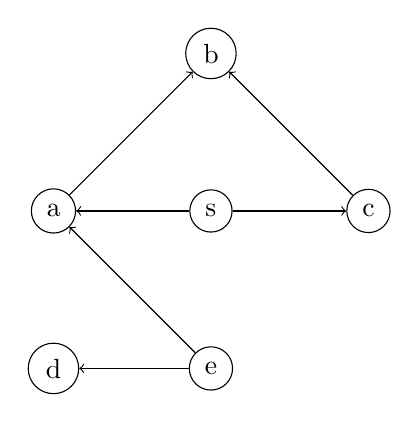
\begin{tikzpicture}[->, auto, node distance=2cm, every node/.style={circle, draw, minimum size=.5cm}]
    \node (s) {s};
    \node (a) [left of=s] {a};
    \node (b) [above of=s] {b};
    \node (c) [right of=s] {c};
    \node (d) [below of=a] {d};
    \node (e) [right of=d] {e};

    \path[every node]
    (s) edge (a)
    (s) edge (c)
    (a) edge (b)
    (c) edge (b)
    (e) edge (d)
    (e) edge (a)
    ;
  \end{tikzpicture}
  \caption{Ein gerichteter Graph}\label{fig:topo}
\end{figure}